% !TeX program = xelatex
% ============================================================
% 1988 年·全国卷·文科 · 试题版
% 由 tools/make_editions.py 生成（重跑会覆盖本文件）；
% 题目/解析内容在 questions.tex / answers*.tex，勿在本文件内写内容。
% ============================================================
\documentclass[zihao=-4, a4paper]{ctexart}
% ============================================================
% common/preamble.tex —— 拆分版试卷项目 · 公共导言区
% 引擎：XeLaTeX；文档类 ctexart 由各版本壳文件自行声明
% 由合并书 math-gaokao-2017-2026/preamble.tex 改造而来：
%   - 页眉左右改为可重定义宏 \gkheadL / \gkheadR（各版本壳设置）
%   - hyperref 不再写死 pdftitle（壳内 \hypersetup 覆盖）
%   - 删除书籍专用的 \chaptermark 重定义与 \gkpaper 装配宏
% ============================================================

% ---------- 数学 ----------
\usepackage{amsmath}
\usepackage{amssymb}
\usepackage{mathtools}

% ---------- 绘图 ----------
\usepackage{tikz}
\usetikzlibrary{shapes.geometric, arrows.meta, calc, patterns, angles, quotes, positioning}
\usepackage{pgfplots}
\pgfplotsset{compat=1.18}

% ---------- 版面 ----------
\usepackage{geometry}
\usepackage{needspace}
\geometry{a4paper, margin=2.2cm, headheight=15pt}
% 紧凑版式（如印刷版）可在壳文件中于 \begin{document} 前再次调用 \geometry 覆盖
\usepackage{enumitem}
\setlist{itemsep=2pt, topsep=4pt, parsep=0pt}

% 中文与行内公式混排的断行弹性：
% emergencystretch 允许段落末路不通时追加伸展量；
% 降低二元/关系符罚分，允许行内长公式在 = 、+ 等处断行（否则整段外溢）
\emergencystretch=2em
\binoppenalty=700
\relpenalty=500
\usepackage{booktabs}      % 三线表
\usepackage[most]{tcolorbox}

% ---------- 选择题选项对齐 ----------
% tasks 宏包：\begin{gkopts}(列数) \task ... \end{gkopts}
% 自动等宽分栏，选项天然对齐；列数已由内容片段按选项长度写定（4/2/1）
\usepackage{tasks}
\settasks{label={}, label-width=0pt, item-indent=1.2em,
          column-sep=1em, after-item-skip=2pt, before-skip=2pt, after-skip=4pt}
\NewTasksEnvironment[style=itemize]{gkopts}[\task](4)

% ---------- 页眉页脚 ----------
\newcommand{\gkheadL}{}   % 左页眉：卷名（壳文件 \renewcommand 设置）
\newcommand{\gkheadR}{}   % 右页眉：版本名（壳文件 \renewcommand 设置）
\usepackage{fancyhdr}
\pagestyle{fancy}
\fancyhf{}
\fancyhead[L]{\small\gkheadL}
\fancyhead[R]{\small\gkheadR}
\fancyfoot[C]{\small —— 第 \thepage\ 页 ——}
\renewcommand{\headrulewidth}{0.4pt}

% ---------- 超链接（须最后加载）----------
\usepackage{hyperref}
\hypersetup{colorlinks=true, linkcolor=blue!55!black,
            bookmarksnumbered=true, unicode=true}

% ============================================================
% common/macros.tex —— 自定义命令与环境（题号、解析头、提示框等）
% 与合并书 math-gaokao-2017-2026/preamble.tex 的自定义段保持一致，
% 保证内容片段（questions.tex / answers.tex）在两个项目间可互换。
% ============================================================

% ---------- 试卷标识（壳文件 \renewcommand 设置，用于 label 命名空间）----------
\newcommand{\gkpaperid}{none}

% ---------- 题号 ----------
% 试题部分的题号：加粗编号 + 自动 \label{q:<卷id>:<题号>}
\newcommand{\gkti}[1]{\par\medskip\noindent
  \textbf{#1．}\phantomsection\label{q:\gkpaperid:#1}\ignorespaces}
% 多卷/分部重启题号时，#1 是唯一内部顺序号（交叉引用身份），#2 才是原卷显示题号。
\newcommand{\gktiwithlabel}[2]{\par\medskip\noindent
  \textbf{#2．}\phantomsection\label{q:\gkpaperid:#1}\ignorespaces}

% 解析部分的题头：小标题 + 回链到试题页
% （仅在题目与解析同文档的版本中回链有效；试题版不含解析头，无悬空引用）
\newcommand{\gksolhead}[2]{%
  \Needspace{3\baselineskip}\subsubsection*{第 #1 题\if\relax\detokenize{#2}\relax\else（#2）\fi}%
  \phantomsection\label{s:\gkpaperid:#1}%
  {\small\color{gray}（题目见第~\pageref{q:\gkpaperid:#1}~页）}\par\nopagebreak}
% 与 \gktiwithlabel 成对：显示原题号，但回链仍用唯一内部顺序号。
\newcommand{\gksolheadwithlabel}[3]{%
  \Needspace{3\baselineskip}\subsubsection*{第 #2 题\if\relax\detokenize{#3}\relax\else（#3）\fi}%
  \phantomsection\label{s:\gkpaperid:#1}%
  {\small\color{gray}（题目见第~\pageref{q:\gkpaperid:#1}~页）}\par\nopagebreak}

% ---------- 填空题空位 ----------
\newcommand{\gkblank}{\underline{\hspace{2.2em}}}

% ---------- 提示框 ----------
% 卷种提示 / 解析归属声明（醒目，浅黄）
\newtcolorbox{gknotice}{colback=yellow!8, colframe=orange!60!black,
  boxrule=0.5pt, arc=1.5pt, left=6pt, right=6pt, top=4pt, bottom=4pt,
  before skip=8pt, after skip=8pt}

% 方法提示 / 注（浅蓝，用于解析后的点评与题量说明）
\newtcolorbox{gktip}{colback=blue!4, colframe=blue!35!black,
  boxrule=0.4pt, arc=1.5pt, left=6pt, right=6pt, top=4pt, bottom=4pt,
  before skip=6pt, after skip=6pt, fontupper=\small}

% ---------- 答案行 ----------
% 解析中独立成段的"答案：X"用带底色的行呈现
\newcommand{\gkanswer}[1]{\par\smallskip\noindent
  \tcbox[width=\linewidth, tcbox width=auto limited,
         colback=green!6, colframe=green!35!black, boxrule=0.4pt,
         arc=1.5pt, left=4pt, right=4pt, top=2pt, bottom=2pt,
         nobeforeafter]{\textbf{#1}}\par\smallskip}

% ---------- 结构标题 ----------
% 结构标题后通常紧跟一个带 0.5\textheight 起始预留的解析题块；0.4 只够放标题，
% 会把下一题整体推到下一页，留下孤立的「二、填空题」等页尾标题。
\newcommand{\gkpart}[1]{\Needspace{0.6\textheight}\subsection*{#1}\nopagebreak}     % 标题 + 首题
% （一）必考题 / 解析小问标题：块式加粗段，可自动换行（\paragraph 的 run-in 版式会溢出）
\newcommand{\gksubpart}[1]{\Needspace{6\baselineskip}\par\medskip\noindent\textbf{#1}\par\nopagebreak\smallskip}

% 罗马数字Ⅰ-Ⅻ（U+2160）与圈号①②③（U+2460）划入 CJK 字符类，
% 用中文字体渲染——西文字体 Latin Modern 缺这些字形，否则整段静默丢字
\xeCJKDeclareCharClass{CJK}{"2160 -> "217F, "2460 -> "24FF}

% ============================================================
% common/questions_env.tex —— 题目 / 解析的语义包装环境
%
% questions.tex 中每道题包在 \begin{question}...\end{question} 里，
% answers.tex 中每题解析包在 \begin{answer}...\end{answer} 里；
% 题头排版仍由内容行中的 \gkti / \gksolhead 完成（见 macros.tex）。
%
% 环境本身不产生任何盒子或垂直间距（只引入一个 TeX 分组），
% 排版结果与不包裹时逐点一致。它的价值在于：
%   1. 给每道题一个机器可数的结构边界（校验脚本数环境数 = 题量）；
%   2. 为将来的条件编译留钩子——某版本可重定义环境实现按题取舍。
% ============================================================

% 环境不把整题装盒：题目与解析仍可自然跨页，但开始题块前必须为题面、
% 图形/表格或解析首段留出足够空间。仅保留 2 个 baseline 会让题干、
% 选项和图形在页边界处被拆开，形成不可打印的孤立内容；题目保留
% 0.15\textheight，在避免短题制造大段空白与避免题块拆分之间取平衡。
% 解析题块保留 0.5\textheight，以容纳“题面 + 图形/选项 + 首段解析”；
% 结构标题仍用更大的保留量；末页自然收尾由视觉复审判定。
\newenvironment{question}{\Needspace{0.15\textheight}}{}
\newenvironment{answer}{\Needspace{0.5\textheight}}{}

\renewcommand{\gkpaperid}{gk-1988-regular-national-arts}
\renewcommand{\gkheadL}{1988 年·全国卷·文科 · 数学}
\renewcommand{\gkheadR}{试题版}
\hypersetup{pdftitle={1988 年·全国卷·文科 数学 · 试题版}}
\begin{document}
\begin{center}
  {\Large\bfseries 1988 年·全国卷·文科}\\[4pt]
  {\large 数学 · 试题版}
\end{center}
\medskip
\pdfbookmark[1]{试题}{sec:q}
% questions.tex —— 1988 年·全国卷·文科 · 题目内容片段（无答案）
% 由 tools/generate_projects.py 依来源总账自 1988/1988_数学真题_全国文_试题.md 生成，勿手改（改源 MD 后重跑）


\gkpart{文科数学}

\begin{gktip}
\textbf{来源说明}：本题面依据固定源 PDF《1988 普通高等学校招生考试（全国卷文）》逐题转录。固定源共 1 页、原卷印刷页码 33；PDF 含题面文字层和矢量图形，但不含答案、解析或评分标准，以下答案和解析由本库独立推导。

\textbf{图形说明}：第 4、12、22 题的函数图象、正四棱台和四棱锥图依据固定源图形关系重绘为 TikZ 矢量图。
\end{gktip}

\begin{question}
\gkti{1}复数

\nopagebreak[4]
\[
\left(\frac{1-i}{1+i}\right)^2
\]

的值等于\mbox{（　　）}

（A）$1$　　（B）$-1$　　（C）$i$　　（D）$-i$

\end{question}
\begin{question}
\gkti{2}圆 $M$ 的方程为

\nopagebreak[4]
\[
(x-3)^2+(y-2)^2=2,
\]

\Needspace{5\baselineskip}
直线 $L$ 的方程为

\nopagebreak[4]
\[
x+y-3=0,
\]

点 $P$ 的坐标为 $(2,1)$，那么\mbox{（　　）}

（A）点 $P$ 在直线 $L$ 上，但不在圆 $M$ 上

（B）点 $P$ 在圆 $M$ 上，但不在直线 $L$ 上

（C）点 $P$ 既在圆 $M$ 上，又在直线 $L$ 上

（D）点 $P$ 既不在直线 $L$ 上，也不在圆 $M$ 上

\end{question}
\begin{question}
\gkti{3}集合 $\{1,2,3\}$ 的子集共有\mbox{（　　）}

（A）5 个　　（B）6 个　　（C）7 个　　（D）8 个

\Needspace{0.4\textheight}
\end{question}
\begin{question}
\gkti{4}函数

\nopagebreak[4]
\[
y=a^x\qquad(0<a<1)
\]

的图象是\mbox{（　　）}
\nopagebreak[4]
\begin{center}% 1988 年全国卷文科第 4 题：指数函数图象的四个选项
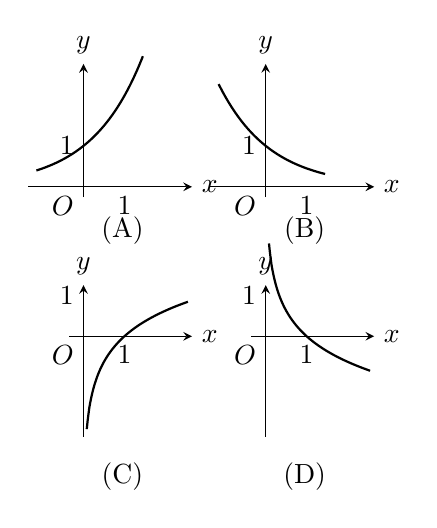
\begin{tikzpicture}[scale=0.52,>=stealth]
  \begin{scope}
    \draw[->] (-1.35,0)--(2.65,0) node[right] {$x$};
    \draw[->] (0,-0.25)--(0,3.0) node[above] {$y$};
    \draw[thick,domain=-1.15:1.45,samples=100]
      plot (\x,{exp(0.8*\x)});
    \node[left] at (0,1) {$1$};
    \node[below] at (1,0) {$1$};
    \node[below left] at (0,0) {$O$};
    \node[below] at (0.95,-0.5) {(A)};
  \end{scope}

  \begin{scope}[xshift=4.45cm]
    \draw[->] (-1.35,0)--(2.65,0) node[right] {$x$};
    \draw[->] (0,-0.25)--(0,3.0) node[above] {$y$};
    \draw[thick,domain=-1.15:1.45,samples=100]
      plot (\x,{exp(-0.8*\x)});
    \node[left] at (0,1) {$1$};
    \node[below] at (1,0) {$1$};
    \node[below left] at (0,0) {$O$};
    \node[below] at (0.95,-0.5) {(B)};
  \end{scope}

  \begin{scope}[yshift=-3.65cm]
    \draw[->] (-0.35,0)--(2.65,0) node[right] {$x$};
    \draw[->] (0,-2.45)--(0,1.25) node[above] {$y$};
    \draw[thick,domain=0.08:2.55,samples=120]
      plot (\x,{0.9*ln(\x)});
    \node[left] at (0,1) {$1$};
    \node[below] at (1,0) {$1$};
    \node[below left] at (0,0) {$O$};
    \node[below] at (0.95,-2.85) {(C)};
  \end{scope}

  \begin{scope}[xshift=4.45cm,yshift=-3.65cm]
    \draw[->] (-0.35,0)--(2.65,0) node[right] {$x$};
    \draw[->] (0,-2.45)--(0,1.25) node[above] {$y$};
    \draw[thick,domain=0.08:2.55,samples=120]
      plot (\x,{-0.9*ln(\x)});
    \node[left] at (0,1) {$1$};
    \node[below] at (1,0) {$1$};
    \node[below left] at (0,0) {$O$};
    \node[below] at (0.95,-2.85) {(D)};
  \end{scope}
\end{tikzpicture}
\end{center}
\nopagebreak[4]
\end{question}
\begin{question}
\gkti{5}已知椭圆方程

\nopagebreak[4]
\[
\frac{x^2}{20}+\frac{y^2}{11}=1,
\]

那么它的焦距是\mbox{（　　）}

（A）$6$　　（B）$3$　　（C）$2\sqrt{31}$　　（D）$\sqrt{31}$

\end{question}
\begin{question}
\gkti{6}在复平面内，与复数

\nopagebreak[4]
\[
z=-1-i
\]

的共轭复数对应的点位于\mbox{（　　）}

（A）第一象限　　（B）第二象限　　（C）第三象限　　（D）第四象限

\end{question}
\begin{question}
\gkti{7}在

\nopagebreak[4]
\[
(x-\sqrt3)^{10}
\]

的展开式中，$x^6$ 的系数是\mbox{（　　）}

（A）$-27C_{10}^{6}$　　（B）$27C_{10}^{4}$

（C）$-9C_{10}^{6}$　　（D）$9C_{10}^{4}$

\end{question}
\begin{question}
\gkti{8}函数

\nopagebreak[4]
\[
y=3\cos\left(\frac25x-\frac\pi6\right)
\]

的最小正周期是\mbox{（　　）}

（A）$\frac25\pi$　　（B）$\frac52\pi$　　（C）$2\pi$　　（D）$5\pi$

\end{question}
\begin{question}
\gkti{9}$\sin\left(-\dfrac{19}{6}\pi\right)$ 的值等于\mbox{（　　）}

（A）$\frac12$　　（B）$-\frac12$　　（C）$\frac{\sqrt3}{2}$　　（D）$-\frac{\sqrt3}{2}$

\end{question}
\begin{question}
\gkti{10}直线

\nopagebreak[4]
\[
x+ay=2a+2
\]

\Needspace{5\baselineskip}
与直线

\nopagebreak[4]
\[
ax+y=a+1
\]

平行（不重合）的充要条件是\mbox{（　　）}

（A）$a=\frac12$　　（B）$a=-\frac12$　　（C）$a=1$　　（D）$a=-1$

\end{question}
\begin{question}
\gkti{11}函数

\nopagebreak[4]
\[
y=\frac{x-2}{2x-1}\qquad\left(x\in R,\ x\ne\frac12\right)
\]

的反函数是\mbox{（　　）}

（A）$y=\frac{x-2}{2x-1}\ (x\in R,\ x\ne\frac12)$

（B）$y=\frac{2x-1}{x-2}\ (x\in R,\ x\ne2)$

（C）$y=\frac{x+2}{2x-1}\ (x\in R,\ x\ne\frac12)$

（D）$y=\frac{2x-1}{x+2}\ (x\in R,\ x\ne-2)$

\Needspace{0.4\textheight}
\end{question}
\begin{question}
\gkti{12}如图，正四棱台中，$A'D'$ 所在的直线与 $BB'$ 所在的直线是\mbox{（　　）}
\nopagebreak[4]
\begin{center}% 1988 年全国卷文科第 12 题：正四棱台
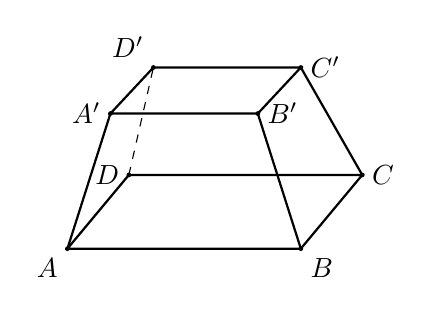
\begin{tikzpicture}[scale=0.78,>=stealth]
  \coordinate (A) at (0,0);
  \coordinate (B) at (3.8,0);
  \coordinate (C) at (4.8,1.2);
  \coordinate (D) at (1.0,1.2);
  \coordinate (Ap) at (0.7,2.2);
  \coordinate (Bp) at (3.1,2.2);
  \coordinate (Cp) at (3.8,2.95);
  \coordinate (Dp) at (1.4,2.95);
  \draw[thick] (A)--(B)--(C)--(D)--cycle;
  \draw[thick] (Ap)--(Bp)--(Cp)--(Dp)--cycle;
  \draw[thick] (A)--(Ap) (B)--(Bp) (C)--(Cp);
  \draw[dashed] (D)--(Dp);
  \fill (A) circle (1.1pt) node[below left] {$A$};
  \fill (B) circle (1.1pt) node[below right] {$B$};
  \fill (C) circle (1.1pt) node[right] {$C$};
  \fill (D) circle (1.1pt) node[left] {$D$};
  \fill (Ap) circle (1.1pt) node[left] {$A'$};
  \fill (Bp) circle (1.1pt) node[right] {$B'$};
  \fill (Cp) circle (1.1pt) node[right] {$C'$};
  \fill (Dp) circle (1.1pt) node[above left] {$D'$};
\end{tikzpicture}
\end{center}
\nopagebreak[4]
（A）相交直线　　（B）平行直线

（C）不互相垂直的异面直线　　（D）互相垂直的异面直线

\end{question}
\begin{question}
\gkti{13}函数

\nopagebreak[4]
\[
y=\sin\left(x+\frac\pi4\right)
\]

在闭区间\mbox{（　　）}上是增函数

（A）$\left[-\frac\pi2,\frac\pi2\right]$　　（B）$\left[-\frac{3\pi}{4},\frac\pi4\right]$

（C）$[-\pi,0]$　　（D）$\left[-\frac\pi4,\frac{3\pi}{4}\right]$

\end{question}
\begin{question}
\gkti{14}假设在 200 件产品中有 3 件次品，现在从中任意抽取 5 件，其中至少有 2 件次品的抽法有\mbox{（　　）}

（A）$C_3^2C_{197}^3+C_3^3C_{197}^2$ 种

（B）$C_3^2C_{197}^3$ 种

（C）$C_{200}^5-C_{197}^5$ 种

（D）$C_{200}^5-C_3^1C_{197}^4$ 种

\end{question}
\begin{question}
\gkti{15}已知二面角 $\alpha-AB-\beta$ 的平面角是锐角 $\theta$，$\alpha$ 内一点 $C$ 到 $\beta$ 的距离为 $3$，点 $C$ 到棱 $AB$ 的距离为 $4$，那么 $\tan\theta$ 的值等于\mbox{（　　）}

（A）$\frac34$　　（B）$\frac35$　　（C）$\frac{3\sqrt7}{7}$　　（D）$\frac{\sqrt7}{3}$

\end{question}
\begin{question}
\gkti{16}求复数

\nopagebreak[4]
\[
\sqrt3-i
\]

的模和辐角的主值。

\end{question}
\begin{question}
\gkti{17}解方程

\nopagebreak[4]
\[
9^{-x}-2\cdot3^{1-x}=27.
\]

\end{question}
\begin{question}
\gkti{18}已知

\nopagebreak[4]
\[
\sin\theta=-\frac35,\qquad
3\pi<\theta<\frac{7\pi}{2},
\]

\Needspace{5\baselineskip}
求

\nopagebreak[4]
\[
\tan\frac\theta2.
\]

\end{question}
\begin{question}
\gkti{19}一个直角三角形的两条直角边的长分别为 $3\text{ cm}$ 和 $4\text{ cm}$，将这个直角三角形以斜边为轴旋转一周，求所得旋转体的体积。

\end{question}
\begin{question}
\gkti{20}求极限

\nopagebreak[4]
\[
\lim_{n\to\infty}\frac{3n^2+2n}{n^2+3n-1}.
\]

\end{question}
\begin{question}
\gkti{21}证明：

\nopagebreak[4]
\[
\cos3\alpha=4\cos^3\alpha-3\cos\alpha.
\]

\Needspace{0.4\textheight}
\end{question}
\begin{question}
\gkti{22}如图，四棱锥 $S-ABCD$ 的底面是边长为 $1$ 的正方形，侧棱 $SB$ 垂直于底面，并且

\nopagebreak[4]
\[
SB=\sqrt3.
\]

用 $\alpha$ 表示 $\angle ASD$，求 $\sin\alpha$。
\nopagebreak[4]
\begin{center}% 1988 年全国卷文科第 22 题：四棱锥 S-ABCD
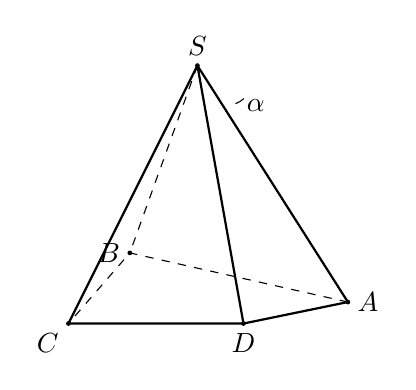
\begin{tikzpicture}[scale=0.78,>=stealth]
  \coordinate (S) at (2.1,4.2);
  \coordinate (B) at (1.0,1.15);
  \coordinate (A) at (4.55,0.35);
  \coordinate (D) at (2.85,0.0);
  \coordinate (C) at (0,0.0);
  \draw[thick] (S)--(C) (S)--(D) (S)--(A);
  \draw[dashed] (S)--(B);
  \draw[thick] (C)--(D)--(A);
  \draw[dashed] (A)--(B)--(C);
  \draw (2.72,3.58) arc (-70:-48:0.42);
  \node at (3.05,3.55) {$\alpha$};
  \fill (S) circle (1.1pt) node[above] {$S$};
  \fill (A) circle (1.1pt) node[right] {$A$};
  \fill (B) circle (1.1pt) node[left] {$B$};
  \fill (C) circle (1.1pt) node[below left] {$C$};
  \fill (D) circle (1.1pt) node[below] {$D$};
\end{tikzpicture}
\end{center}
\nopagebreak[4]
\end{question}
\begin{question}
\gkti{23}在双曲线

\nopagebreak[4]
\[
x^2-y^2=1
\]

的右支上求点 $P(a,b)$，使该点到直线 $y=x$ 的距离为 $\sqrt2$。

\end{question}
\begin{question}
\gkti{24}解不等式：

\nopagebreak[4]
\[
\lg\left(x-\frac1x\right)<0.
\]

\end{question}
\begin{question}
\gkti{25}一个数列 $\{a_n\}$：当 $n$ 为奇数时，

\nopagebreak[4]
\[
a_n=5n+1;
\]

\Needspace{5\baselineskip}
当 $n$ 为偶数时，

\nopagebreak[4]
\[
a_n=2^{n/2}.
\]

求这个数列的前 $2m$ 项的和（$m$ 是正整数）。

\end{question}
\end{document}
